\documentclass[a4paper]{article}

%% Language and font encodings
\usepackage[utf8x]{inputenc}
\usepackage[T1]{fontenc}
\usepackage[ngerman]{babel}

%% Sets page size and margins
\usepackage[a4paper,top=3cm,bottom=2cm,left=3cm,right=3cm,marginparwidth=1.75cm]{geometry}
\setlength{\parindent}{0pt}

%% Useful packages
\usepackage{amsmath}
\usepackage{amssymb}

\usepackage{mathrsfs}
\usepackage{graphicx}
\usepackage[colorinlistoftodos]{todonotes}
\usepackage[colorlinks=true, allcolors=blue]{hyperref}
\newcommand{\ff}[1]{\mathscr{F}\left[#1\right]}

\title{Mathematischer Hintergrund und Variablenbenennung}
\author{Simon Jung, Bernd Lienau, Alexander Franke}
\date{\today}
\begin{document}
\maketitle

\section{Ebene Welle}
Wir betrachten zunächst eine einfache ebene Welle. Diese laufe in $z$-Richtung. Wir erhalten also für das elektrische Feld $E(z,t)$
\begin{align}
E(z,t) = E_0 \cdot \sin(k z-\omega t)
\end{align}

Bzw. unter Verwendung der Frequenz $\nu$ und ohne den Wellenvektor $|\vec{k}| := k = \frac{\omega}{c} = \frac{2\pi}{\lambda}$

\begin{align}
E(z,t) &= E_0 \cdot \sin (\frac{2\pi\nu}{c} z - 2\pi\nu t ) \\
\Rightarrow E(z,t) &= E_0 \sin\left((2\pi\nu \left(\frac{z}{c} - t\right)\right)
\end{align}
 Für das menschliche Auge ist nur die Intensität des Lichts bedeutsam. Sie ist proportional zum Quadrat der
elektrischen Feldstärke der Lichtwelle: 
\begin{align}
I_\text{Licht} \propto E^2 
\end{align}
\section{Beugung an einfachen Objekten}
\subsection{Vorüberlegungen zum Einzelspalt}
Wir definieren unseren Einzelspalt (und später unser Gitter) auf den Punkt $z=0$. Die Betrachtung des Beugungsmusters ist im Abstand $z_\text{Schirm}$ oder kurz $z_S$ dahinter. 
Unsere Spaltgröße ist definiert als $a$, ähnlich später unsere Gitterkonstante $a$. Wir verwenden Frauenhofer Beugung ($z_S \gg a$). Frauenhofer Beugung verlangt außerdem, dass eine ebene Welle auf den Spalt trifft.

Wir definieren als weitere Dimension für den Schirm die x-Achse ("nach oben und unten")  um konform mit einem Linkshand-Koordinatensystem zu sein. Die Maxima auf dem Schirm werden entsprechend $s_0, s_{+1}, s_{-1}, s_{+2}$ genannt.

Um das Wellenfeld beim Schirm $z_S$ zu erhalten, müssen wir nun
nach dem Huygens‘schen Prinzip alle Elementarwellen aus dem Spalt am Betrachtungsort
überlagern, d. h. die Summe der entsprechenden Felder bilden.

Mit dem Übergang zur komplexen Darstellung und Überlagerung von $N$ Wellen:
\begin{align}
E(z,t) &= E_0 \Big[ e^{i(k z-\omega t)} + e^{i(k (z+\Delta)-\omega t)} + e^{i(k (z+2\Delta)-\omega t)} + \dots + e^{i(k (z+(N-1)\Delta)-\omega t)} \Big] \\
&= E_0  e^{k z-\omega t} \Big[ 1 +e^{i\Delta} + e^{i2\Delta} + \dots + e^{i(N-1)\Delta}\Big]
\end{align}
Der Term in der eckigen Klammer lässt sich mit der geometrischen Reihe zur $\frac{\sin(\zeta)}{\zeta}$ Funktion umschreiben.
Die Intensität am Schirm ergibt sich nach Quadrierung zu 
\begin{align}
I_S = I_0 \left( \frac{\sin\left(\frac{\pi a}{\lambda}\sin \alpha_x\right)}{\frac{\pi a}{\lambda} \sin \alpha_x} \right)^2
\label{eq:einzelspalt_vorueberlegung}
\end{align}
Diese Formel sei nur später zur Verifizierung anzuwenden. Das Beugungsmuster in Frauenhoferbeugung ist nämlich allgemein durch die zweidimensionale Fouriertransformation der Amplitudentransmissionfunktion $f(z,x)$ des Beugungsobjektes gegeben. Es lässt sich mit der Fouriertransformation auch viel leichter simulieren wie das Beugungsmuster sich bei Defekten/Fehlstellen im Beugungsobjekt verändert.
\begin{figure}[!htb]
\centering
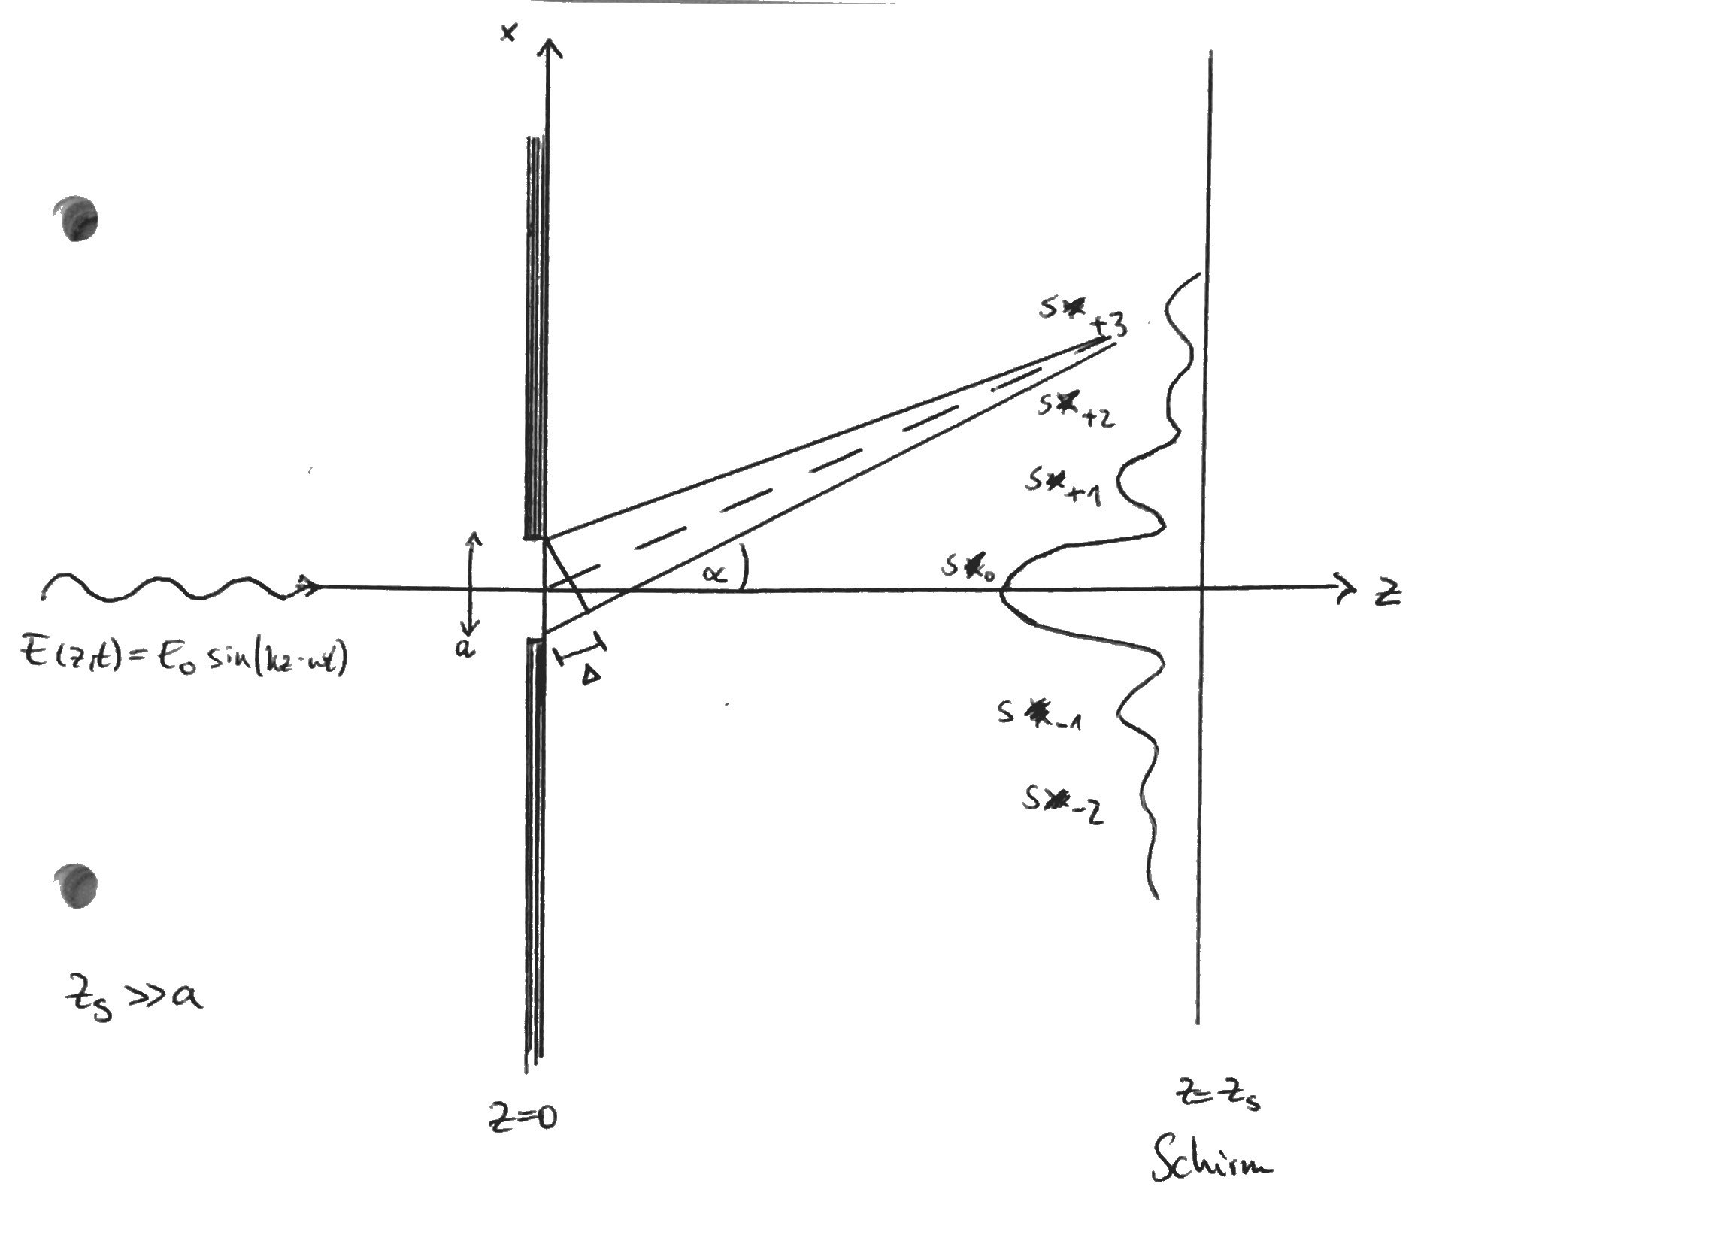
\includegraphics[width=\textwidth]{einzelspalt.pdf}
\caption{Skizze mit allen relevanten Variablen für den Einzelspalt}
\end{figure}

\subsection{Beugungsbilder}
Allgemein ist die Wellenfunktion des Beugungsbildes gegeben durch

\begin{align}
\Psi (u,v) = \int \int f(x,y) \exp\Big(-i(ux+vy)\Big) dx dy
\label{eq:wellenfkt_beugungsbild}
\end{align}
wobei $u= k_0 \sin\alpha_x$ und $v=k_0\sin\alpha_y$
\subsubsection{Einzelspalt}
Wir können unseren Einzelspalt mit der Transmissionsfunktion $f(x,y)$ beschreiben. Wir zerlegen diese Funktion in eine Faltung von Funktionen von $x$ und $y$
\begin{align}
g(x) = \begin{cases} 
1  &\text{für } |x| <  \frac{a}{2} \\
0 & \text{sonst}\end{cases}
\label{eq:einzelspalt}
\end{align}
\begin{align}
h(y) = 1
\end{align}
Wir haben einen Spalt der Dicke a, der in y-Richtung unendlich weit ausgedehnt ist.
Die Faltung dieser beiden Funktionen ist nach dem Faltungstheorem das Produkt der Fouriertransformationen.

Wir finden also für unsere Wellenfunktion nach dem Spalt
\begin{align}
\Psi(\alpha_x,\alpha_y) &= \int_{-a/2}^{a/2} e^{-ixk\sin(\alpha_x)} dx \int_{-\infty}^\infty e^{-iyk\sin(\alpha_y)}dy\\
&= a \frac{\sin(\frac{1}{2} ak\sin(\alpha_x))}{\frac{1}{2} ak\sin(\alpha_x)}\delta\Big(k \sin(\alpha_y)\Big)\\
&= a \frac{\sin( \frac{a\pi}{\lambda} \sin(\alpha_x))}{\frac{a\pi}{\lambda} \sin(\alpha_x)}\delta\Big(k \sin(\alpha_y)\Big)
\end{align}
Mit der Dirac-Funktion $\delta$. Vergleiche mit Gleichung \ref{eq:einzelspalt_vorueberlegung}.

Die Intensitätsverteilungen ergeben sich immer aus:
\begin{align}
I(u,v) &= |\Psi(u,v)|^2\\
\text{beim Einzelspalt: \quad}
|\Psi(u,v)|^2 &= |\Psi(u,0)|^2 
\end{align}
\subsubsection{Beugung an einer Rechteckblende}
Nur als kurzes Beispiel: Ein kleines rechteckiges Loch der Höhe $h$ und Breite $b$ würde sehr ähnlich zu oben ergeben:
\begin{align}
\Psi(\alpha_x,\alpha_y) &= g(x) \cdot h(y) \\
&= \int_{-b/2}^{b/2} e^{-ixk\sin(\alpha_x)} dx \int_{-h/2}^{h/2} e^{-iyk\sin(\alpha_y)}dy\\
&= bh \frac{\sin(\frac{1}{2} bk\sin(\alpha_x))}{\frac{1}{2} bk\sin(\alpha_x)} \cdot \frac{\sin(\frac{1}{2} hk\sin(\alpha_x))}{\frac{1}{2} hk\sin(\alpha_x)}\\
\end{align}
\subsubsection{Beugung an einer Lochblende}
Wir führen natürlich Polarkoordinaten ein. Für die Lochblende haben wir
\begin{align}
x= \rho \cos \theta \qquad y = \rho \sin \theta
\end{align}

Für unser Beugungsmuster (auch rotationssymmetrisch) haben wir den Koordinatensatz:
\begin{align}
x= \xi \cos \phi \qquad y= \xi \sin \phi
\end{align}
Die Lochblende habe den Radius $R$.

Wir erhalten aus Gleichung \ref{eq:wellenfkt_beugungsbild}
\begin{align}
\Psi(u,v)=\Psi(\alpha_x,\alpha_y) = \int_0^R \int_0^{2\pi} \exp\Big[ -i (\rho \xi \cos\phi\cos\theta + \rho\xi\sin\phi\sin\theta) \Big] \rho d\rho d\theta
\end{align}

Dieses Integral kann man mit den Besselfunktionen lösen oder halt mit Numerik, was wir tun werden.
Zur Kontrolle. Das Ergebnis ergibt sich zu:
\begin{align}
\Psi (\xi,\phi ) = \pi R^2 \left( \frac{2J_1(\xi R)}{\xi R} \right)
\end{align}
mit 
\begin{align}
J_{1}(x)=\sum _{{r=0}}^{\infty }{\frac  {(-1)^{r}({\frac  {x}{2}})^{{2r+1 }}}{\Gamma (1 +r+1)r!}}\, 
\end{align}
\subsection{Überlagerung von Beugungsmustern}
Aufgrund der Eigenschaften der Fouriertransformierten, können wir die Überlagerung von Beugungsmustern als algebrische Summe der Transmissionsfunktion einfacher Objekte aufschreiben. Im Allgemeinen muss bei der Transformierten des Gesamtobjektes, Real- und Imaginärteil getrennt addiert werden. Nur für den Sonderfall von Punktsymmetrie bezüglich der Mitte sind die Transformierten reell. 

Beispielsweise kann bei drei Spalten das Beugungsmuster der beiden äußeren zu dem inneren hinzuaddieren. Bei 4 Spalten die beiden inneren zu den äußeren beiden (die äußeren haben den dreifachen Abstand wie die beiden inneren).
\section{Interferenz}
\subsection{Doppelspalt}
\begin{figure}[!htb]
\centering

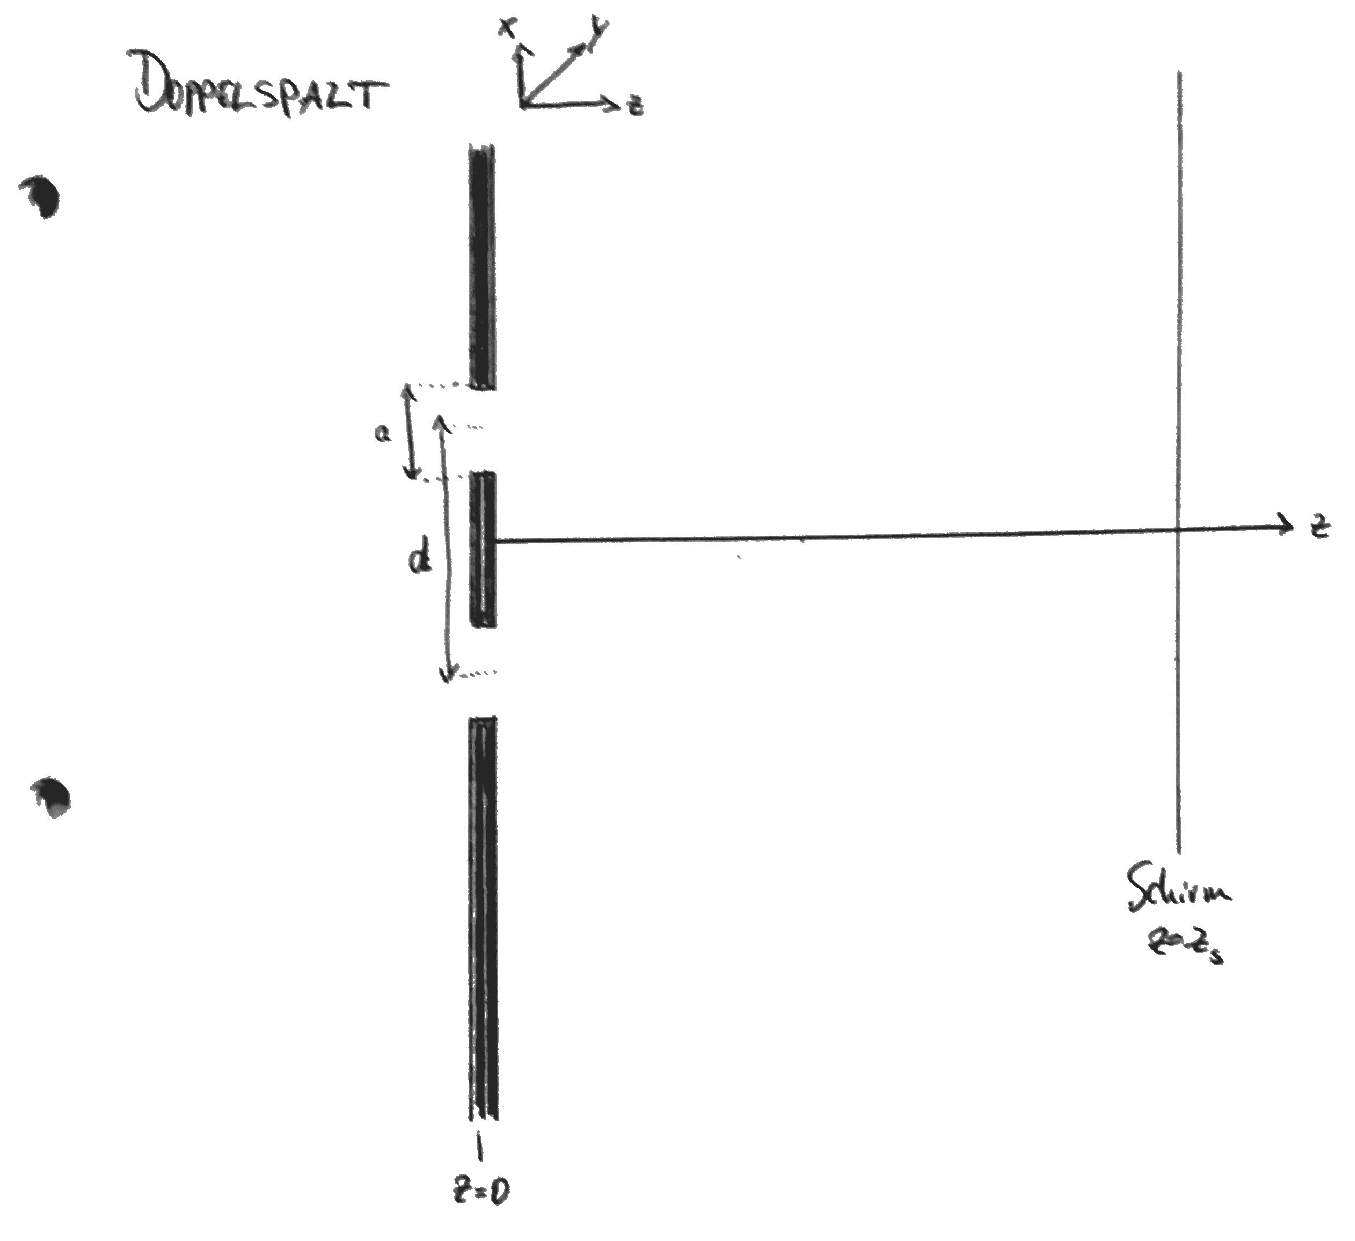
\includegraphics[width=0.5\textwidth]{doppelspalt.pdf}
\end{figure}
Wir betrachten nun die Überlagerung der beiden Beugungsmuster der Einzelspalte. Die Eigenschaften der Fouriertransformation machen dieses Vorgehen sehr viel einfacher, da wir wissen, dass
\begin{align}
g(x) \circledast h(y) = \mathscr{F}[g(x)] \cdot \mathscr{F}[h(y)] \\
\end{align}

Aus Gleichung \ref{eq:einzelspalt} kennen wir die mathematische Beschreibung eines Einzelspaltes der Breite $a$. Wir nehmen nun an das wir zwei Spalte im Abstand $d$ haben. Wir finden also für unsere Gesamtheit mithilfe von zwei Dirac-Deltafunktionen.
\begin{align}
f_{\text{DS}}(x) &= \Bigg[ \delta\left(x-\frac{d}{2}\right) + \delta\left(x+\frac{d}{2}\right) \Bigg]  \circledast f_\text{ES} \\
\Rightarrow \ff{f_{\text{DS}}(x) } &= \ff{ \delta\left(x-\frac{d}{2}\right) + \delta\left(x+\frac{d}{2}\right)  } \cdot \ff{f_\text{ES}}
\end{align}
Wir sollten durch unsere Simulation zu folgendem Ergebnis kommen:
\begin{align}
I(\alpha_x,0) = |\Psi(\alpha_x,0)|^2 =  \cos^2 \left(\frac{\pi d \sin(\alpha_x)}{\lambda}\right) \frac{\sin^2(\pi a \sin(\alpha_x)/\lambda)}{(\pi a \sin(\alpha)/\lambda)^2}
\end{align}
\end{document}